\section{Theorie}
\label{sec:Theorie}

\subsection{Einleitung}
\label{subsec:Einleitung}

Die im folgenden dargestellte Untersuchung eines Reinst-Germanium-Detektors hat im wesentlichen zwei Ziele.
Zum einen sollen charakteristische Eigenschaften des Detektors, wie die Effizienz und das Energieauflösungsvermögen bestimmt werden.
Zum anderen soll der Germanium-Detektor eingesetzt werden, um die Aktivität einer Probe eines unbekannten Materials zu bestimmen und, um Glieder der Zerfallsreihe einer weiteren Probe zu identifizieren.
Der hier verwendete Detektor ist als Instrument der Gamma-Spektroskopie für den Nachweis von bei Kernzerfällen entstehenden Photonen, welche auch Gamma-Quanten genannt werden, entwickelt worden.
Im Gegensatz zu den übrigen Kapiteln wird in Kapitel \ref{subsec:t1} von Photonen statt von Gamma-Quanten gesprochen, um die allgemeine Gültigkeit der dort getätigten Aussagen nicht zu beschränken.

\subsection{Gamma-Strahlung in Materie}
\label{subsec:t1}
Diese Strahlung kann auf verschiedene Weise mit den Elektronen sowie Atomkernen in Materie
interagieren.\\
Jeder Wechselwirkung lässt sich ein sogenannter Wirkungsquerschnitt
$\sigma$ zuordnen. Dieser ist ein Maß für die Wahrscheinlichkeit,
dass der jeweilige Prozess auftritt. Weiter lässt sich damit der sogenannte Extinktionskoeffizient $\mu$ definieren.
Für diesen gilt

\begin{equation}
  \label{eqn:extinktion}
  \mu = \sigma \cdot n .
\end{equation}
Dabei bezeichnet $n$ die Atomdichte pro Volumen des Absorbers.\\
In Abbildung \ref{fig:extinktion} ist die Energieabhängigkeit des Extinktionskoeffizienten für Photoeffekt, Comptoneffekt
und Elektronenpaarbildung gezeigt.
Die Wahrscheinlichkeit für den jeweiligen Prozess, lässt sich dann mithilfe des Extinktionskoeffizenten als

\begin{equation}
  \label{eqn:wkeit}
  w = 1 - e^{-\mu \cdot D}
\end{equation}
bestimmen. Aus eqref{eqn:wkeit} folgt das Absorptionsgesetz
\begin{equation}
  \label{eqn:absorption}
  N(D) = N_{0} \cdot e^{-\mu \cdot D}.
\end{equation}
Dabei bezeichnet $D$ die Dicke des Absorbers. Das Absorptionsgesetz gibt an, wie viele Photonen
noch nicht mit der Materie in Wechselwirkung getreten sind.\\ \\
Bei bei der Interaktion von Gamma-Strahlung mit Elektronen und Atomkernen sind vor allem
der Photoeffekt, der Comptoneffekt und die Paarbildung relevante
Prozesse. Auf diese wird im Folgenden näher eingegangen.\\ \\
Beim Photoeffekt gibt das Photon seine Energie vollständig an ein Hüllenelektron ab, was bei
einer Photonenergie oberhalb der Bindungsenergie des Elektrons dafür sorgt, dass das Elektron
aus seinem Energiezustand entfernt werden kann. Überschüssige Energie bleibt als kinetische
Energie des ausgelösten Elektrons erhalten. Die Unterbesetzung der Schale, der das ausgelöste
Elektron enstammte, wird ausgeglichen, indem ein Elektron aus einer energetisch höheren Schale
die unvollständige Schale auffüllt. Dabei gibt das nachrückende Elektron seine Energie
in Form von Röntgenstrahlung ab. Für den dem Photoeffekt zugeordneten Wirkungsquerschnitt $\sigma_\text{ph}$ gilt

\begin{equation}
  \label{eqn:phquerschnitt}
  \sigma_\text{ph} \propto z^{\alpha} \cdot E^{\delta}.
\end{equation}
Dabei bezeichnet $z$ die Kernladungszahl des Absorbers, $\alpha$ und $\delta$ Paramter, die sich je nach konkretem Anwendungsfall
ändern und $E$ die Energie des Photons. Bei Energien unterhalb von $\SI{5}{\mega\electronvolt}$ liegt $\alpha$ zwischen den Zahlen
$4$ und $5$ und $\delta$ nimmt einen Wert von ca. $-3.5$ an.\\ \\
Der Comptoneffekt beschreibt die inelastische Streuung von Photonen, deren Energie im Bereich von ca.
$\SI{0.01}{\mega\electronvolt}$ bis $\SI{10}{\mega\electronvolt}$ mit einem
ruhenden Elektron.\\
Dabei wird ein vom Streuwinkel $\psi_{\gamma}$ abhängiger Energieanteil an das Elektron übertragen.
Der maximale Energieübertrag findet bei der Rückstreuung also einem Streuwinkel
von $\SI{180}{\degree}$ statt. Es wird die Energie

\begin{equation}
  \label{eqn:comptonuebertrag}
  E_\text{l} = E_{\gamma} \cdot \frac{\varepsilon \left( 1 - \cos\left( \psi_{\gamma} \right) \right)}{1
  + \varepsilon \left( 1 - \cos\left( \psi_{\gamma} \right) \right)}
\end{equation}
übertragen. Dabei bezeichnet $\varepsilon$ den Anteil der ursprünglichen
Photonenergie $E_{\gamma}$ an der Ruheenergie des Elektrons. Der maximale Energieübertrag $E_\text{l,max}$ ist durch

\begin{equation}
  \label{eqn:ckante}
  E_\text{l,max} = E_\gamma \cdot \frac{2\varepsilon}{1 + 2\varepsilon}
\end{equation}
gegeben. Bei der Gammaspektroskopie wird dieser Wert als Compton-Kante bezeichnet.\\
Für den Wirkungsquerschnitt $\sigma_\text{compton}$ ergibt sich

\begin{equation}
  \label{eqn:comptonquerschnitt}
  \sigma_\text{compton} = \frac{3}{4} \cdot \sigma_\text{Th}
  \cdot \left( \frac{1 + \varepsilon}{\varepsilon^2}
  \cdot \left( \frac{2 + 2\varepsilon}{1 + 2\varepsilon} - \varepsilon^{-1} \ln\left( 1 + 2\varepsilon \right) \right)
  + \frac{1}{2\varepsilon} \ln\left( 1 + 2\varepsilon \right) - \frac{1 + 3\varepsilon}{(1 + 2\varepsilon)^2}  \right) .
\end{equation}
Wird $\varepsilon$ beliebig klein, so ergibt sich der Wirkungsquerschnitt nach Thomson
$\sigma_\text{Th}$. Für diesen lässt sich der Streuprozess als elastisch charakterisieren.\\
Es lässt sich zeigen, dass $\sigma_\text{compton}$ sich folgendermaßen mit der Energie, der gestoßenen Elektronen ändert

\begin{equation}
  \label{eqn:dsig}
  \frac{\mathrm{d}\sigma_\text{compton}}{\mathrm{d}E} = \frac{3}{8} \sigma_\text{Th}
  \cdot \frac{1}{m_{0} c^2 \varepsilon^2} \cdot \left(  2 + \left( \frac{E}{h\nu - E} \right)^2
  \cdot \left( \frac{1}{\varepsilon^2} + \frac{h\nu - E}{h\nu} - \frac{2}{\varepsilon}
  \cdot \left( \frac{h\nu - E}{h\nu} \right) \right) \right) .
\end{equation}
\\ \\
Bei der Elektronen-Paarbildung wird aus der Energie eines Photons ein Elektron und ein Positron erzeugt.\\
Damit dies möglich ist, muss die Energie des Photons mindestens doppelt so groß wie die Ruhemasse eines Elektrons
sein. Weiterhin muss der Prozess in Beisein eines Atomkerns oder Elektrons stattfinden. Damit in letzterem Fall
die Paarbildung stattfinden kann muss die Photonergie die vierfache Ruhemasse eines Elektrons überschreiten.
Aufgrund des vergleichsweise hohen Schwellenwerts für das Stattfinden dieses Prozesses, ist dieser offensichtlich erst bei sehr Energien im
Bereich einiger $\si{\mega\electronvolt}$ von Bedeutung.\\
Der Wirkungsquerschnitt für die Paarbildung hat folgende Gestalt
\begin{equation}
  \label{eqn:paarbildung}
  \sigma_\text{Pa} = \alpha \cdot r_\text{e}^2 \cdot z^2 \cdot \left( \frac{28}{9} \cdot \ln\left( \epsilon \right) - \frac{218}{27} \right)
\end{equation}

\begin{figure}
  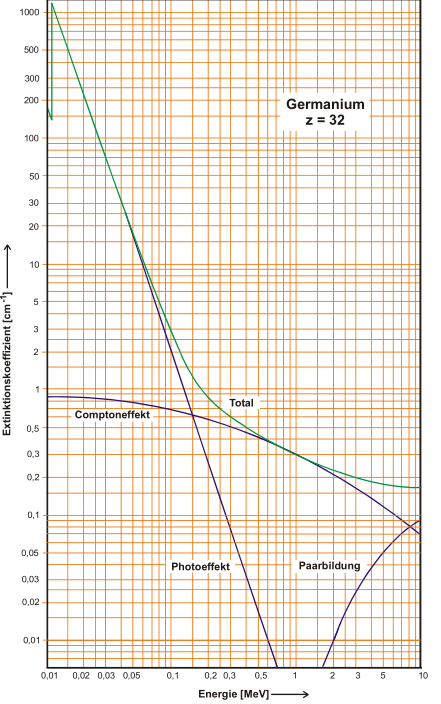
\includegraphics[width=\textwidth]{content/skizzen/extinktion.png}
  \caption{Energieabhängigkeit der Extinktionskoeffizienten der betrachteten Prozesse bei der Wechselwirkung von Gamma-Strahlung mit Materie \cite{sample}.}
  \label{fig:extinktion}
\end{figure}
\FloatBarrier

\subsection{Reinst-Germanium-Detektoren}
\label{subsec:Wirkungsweise}
Das wichtigste Element des Germanium-Detektors ist eine Halbleiterdiode.
Die durch p- bzw. n-Dotierung entstehenden Ladungsträger diffundieren und rekombinieren an der Grenzfläche zwischen den beiden Bereichen der Diode.
Dadurch entsteht um die Grenzfläche herum eine ladungsarme Zone.
Diese Zone ist für die Messung von Gamma-Quanten der entscheidende Bereich der Diode.
Erzeugt ein $Gamma$-Quant innerhalb der Diode ein freies Elektron, zum Beispiel indem mithilfe des Photoeffekts ein Elektron aus dem Valenz- in das Leitungsband gehoben wird, so hebt dieses freie Elektron durch Abgabe seiner kinetischen Energie weitere Elektronen in das Leitungsband.
Entsteht so ein Elektronenschauer in dem positiv oder negativ geladenen Bereich der Diode, wird er durch Rekombination mit den jeweiligen Ladungsträgern des Bereichs eliminiert, und ist damit nicht messbar.
Falls der Elektronenschauer in der ladungsarmen Zone entsteht, gelingt es durch ein hinreichend großes elektrisches Feld, die freien Elektronen von den zurückgelassenen positiv geladenen Atomrümpfen zu trennen, und es entsteht ein Strom $\frac{dQ}{dt}$.
Die Gesamtladung $Q$ ist dabei proportional zur Energie des $Gamma$-Quants, welches den Elektronenschauer verursacht hat, da sie ihrerseits proportional zur Anzahl der Elektronen des Schauers ist.
Ein Ziel bei der Konstruktion eines Germanium-Detektors ist es also, eine möglichst breite ladungsarme Zone zu erreichen.
Dies ist zum Beispiel durch ein starkes elektrisches Feld und eine unsymmetische Dotierung möglich.
Aufgrund der thermischen Bewegungen von Elektronen im Material entsteht ein Rauschen, welches die Messung negativ beeinflusst.
Ein starkes elektrisches Feld zeichnet eine Bewegungsrichtung für die thermische Bewegung der Elektronen aus, was zu einem stärkeren Rauschen führt.
Um diesen Einfluss zu verringern werden Germanium-Detektoren in der Regel auf $\SI{77}{\kelvin}$ gekühlt.

Wichtige Kenngrößen eines Germanium-Detektors sind das energetische Auflösungsvermögen und die Effizienz.
Das energetische Auflösungsvermögen wird größtenteils von der Halbwertsbreite $\Delta E_{\frac{1}{2}}$ eines Peaks des Spektrums beschrieben.
Wie Abbildung \ref{fig:halbwertsbreite} zeigt, können zwei benachbarte Spektrallinien hinreichend gut unterschieden werden, wenn der Abstand zwischen ihnen mindestens der Halbwertsbreite entspricht.
\begin{figure}
\centering
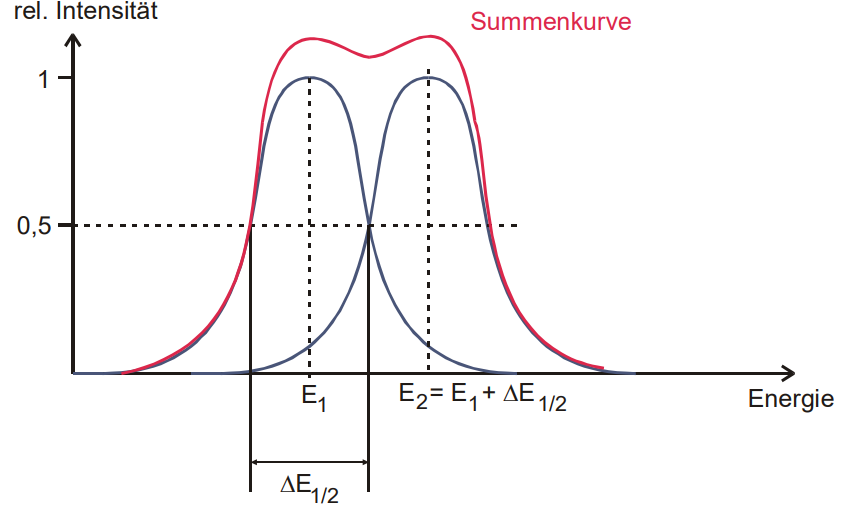
\includegraphics[width=0.8\textwidth]{content/skizzen/halbwertsbreite.png}
\caption{Durch die Überlagerung zweier Gaußkurven wird die Unterscheidbarkeit von zwei verschiedenen Spektrallinien dargestellt.}
\label{fig:halbwertsbreite}
\end{figure}
Die Halbwertsbreite wird von der Anzahl $n$ der nach Einfall eines Gamma-Quants freigesetzten Elektron-Loch-Paare bestimmt.
Da typischer Weise $n\gg 1$ beobachtet wird, kann die Verteilungsfunktion durch eine Gauß-Verteilung angenähert werden.
Ist $\sigma_E$ die Standardabweichung der Gauß-Verteilung, so gilt für die Halbwertsbreite
\begin{align}
\Delta E_{\frac{1}{2}} = \sqrt{8 \text{ln} ~2} \sigma_E \approx 2,35 \cdot \sqrt{0,1 \cdot E_{\gamma} E_{\text{EL}}} \text{ ,}
\label{eq:t:halbwertsbreite}
\end{align}
wobei $E_{\gamma}$ die Energie des einfallenden Gamma-Quants, $E_{\text{EL}}$ die Bindungsenergie eines Elektron-Loch-Paars und $0,1$ der sogenannte Fano-Faktor ist.
Weitere Faktoren sind unter anderem der Leckstrom, Inhomogenitäten des elektrischen Feldes oder das Verstärkerrauschen.
Jeder dieser Faktoren kann durch geeignete Gegenmaßnahmen verringert werden.
Etwa durch Kühlung der Apparatur, hohe Spannungen und Vergrößerung des Detektors.
Das energetische Auflösungsvermögen hängt neben der Halbwertsbreite der oben diskutierten Verteilung mittels
\begin{align}
H_\text{ges}^2 = \Delta E_{\frac{1}{2}}^2 + H_\text{R}^2 + H_\text{I}^2 + H_\text{E}^2
\end{align}
von den Halbwertsbreiten ab, welche durch den Leckstrom ($H_\text{R}$), die Feldinhomogenität ($H_\text{I}$) und das Verstärkerrauschen ($H_\text{E}$) enstehen.
Die Effizienz beschreibt die Abhängigkeit der Vollenergie-Nachweiswahrscheinlichkeit eines Detektors von der Energie der einfallenden Gamma-Quanten.
Für den Nachweis der Gesamtenergie eines Gamma-Quants im Detektor kommt von den in Kapitel \ref{subsec:t1} behandelten Phänomenen nur der Photoeffekt in Frage.
Gleichung \eqref{eqn:phquerschnitt} ist anzusehen, dass die Effizienz bei zunehmender Energie $E_{\gamma}$ der Gamma-Quanten stark abfällt.

\subsection{Elektronische Beschaltung eines Germanium-Detektors}
\label{subsec:Elektronische Beschaltung eines Germanium-Detektors}
Der Detektor erzeugt für ein einfallendes Teilchen eine Ladungsänderung $\frac{dQ}{dt}$, welche als Strom gemessen werden kann.
Ziel der elektronischen Beschaltung des Detektors ist es nun diesen Strom in einen Spannungsimpuls proportional zur Energie $E_\gamma$ des Teilchens zu erzeugen und diesen geeignet zu speichern.
Um den Strom in eine Spannung umzuwandeln wird er im Vorverstärker mittels einer Integrationsstufe integriert (vgl. Abbildung \ref{fig:t:1}).
\begin{figure}
\centering
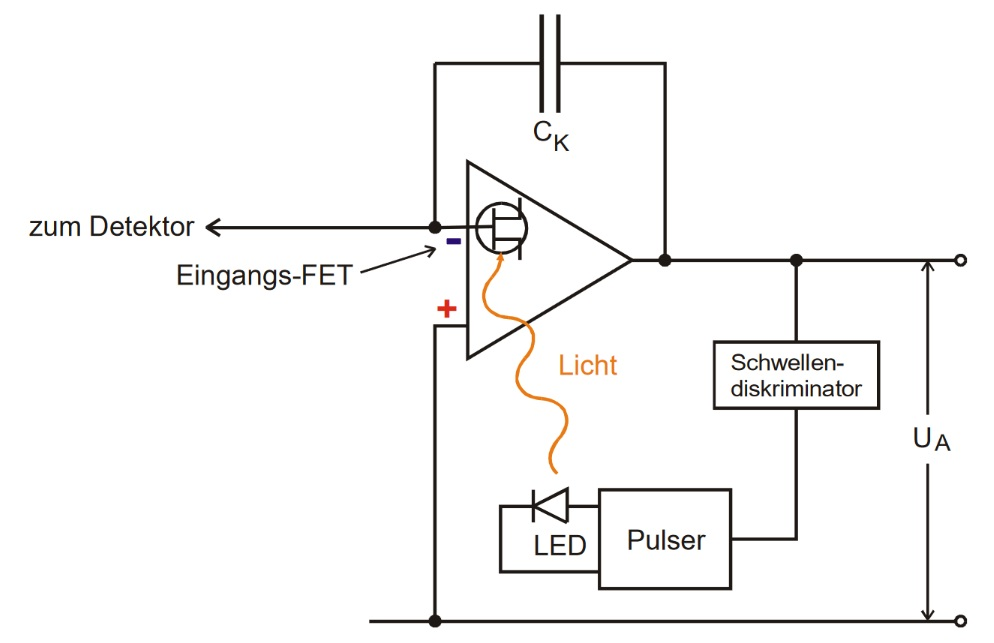
\includegraphics[width=0.8\textwidth]{content/skizzen/aufbau2.jpg}
\caption{Schaltbild des Vorverstärkers \cite{sample}.}
\label{fig:t:1}
\end{figure}
Damit sich die Spannungen verschiedener Signale nicht addieren muss der Kondensator des Vorverstärkers nach der Detektion eines Signals entladen werden.
Dafür sorgt eine rauscharme optoelektronische Rückkopplung.
Die Spannungssignale müssen nun ihrer Höhe nach geordnet abgespeichert werden.
Ein in Abbildung \ref{fig:t:2} schematisch dargestellter Wilkinson-Analog-Digital-Converter (ADC) ordnet jedem Spannungssignal eine Zahl zu, welche die Höhe des Signals repräsentiert.
\begin{figure}
\centering
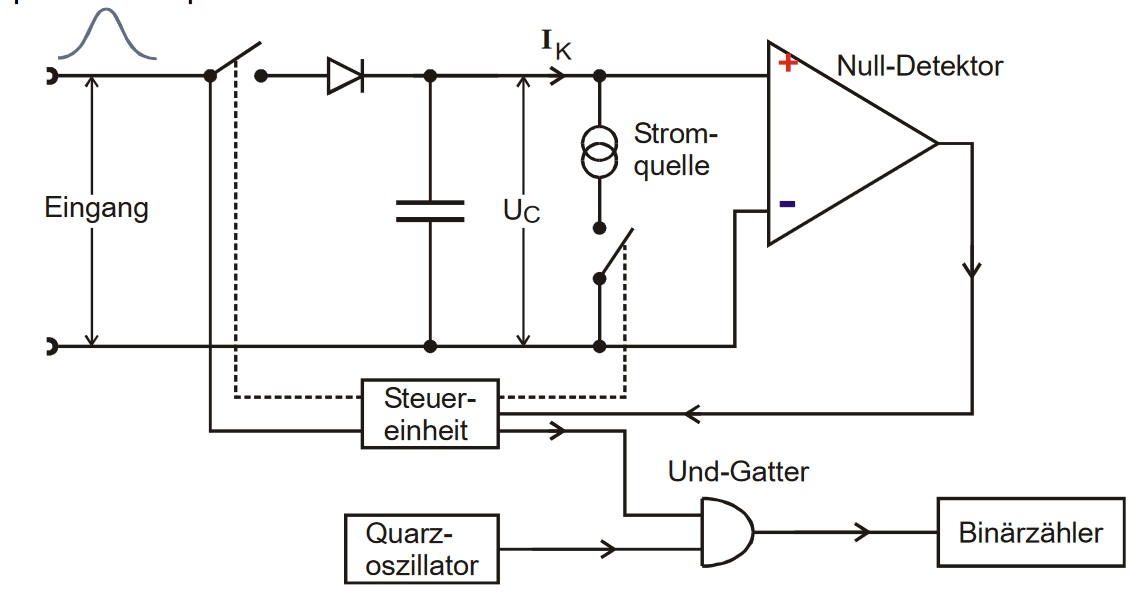
\includegraphics[width=0.8\textwidth]{content/skizzen/aufbau3.jpg}
\caption{Aufbau eines Wilkinson-Analog-Digital-Converters \cite{sample}.}
\label{fig:t:2}
\end{figure}
Dazu wird ein Kondensator mit dem vom Vorverstärker kommenden Signal geladen und mit einem konstanten Strom entladen.
Eine Zeitmesseinheit zählt die Zeit bis der Kondensator vollständig entladen ist.
Dieses digitale Signal wird von einem Vielkanalanalysator in einem dem Zählergebnis zugeordneten Kanal gespeichert.
Die Anzahl der Signale, die in einem bestimmten Kanal gespeichert werden, entspricht also der Häufigkeit des Auftretens eines Signals mit dieser Energie.
Ein Schaubild der gesamten Schaltung ist in Abbildung \ref{fig:t:3} dargestellt.
\begin{figure}
\centering
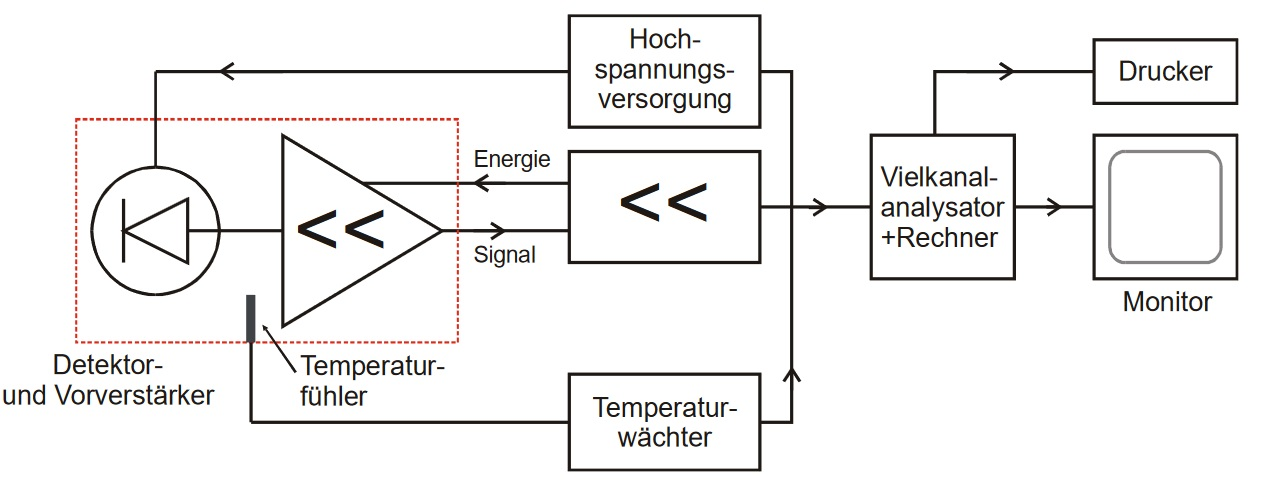
\includegraphics[width=0.8\textwidth]{content/skizzen/aufbau4.jpg}
\caption{Elektronische Beschaltung eines Germanium-Detektors \cite{sample}.}
\label{fig:t:3}
\end{figure}
Das Ergebnis kann zum Beispiel in einem Balkendiagramm gezeichnet werden und entspricht dann dem $Gamma$-Spektrum der radioaktiven Probe.


\subsection{Das zu messende Spektrum eines Gammastrahlers}
\label{subsec:spektrum}

Nimmt man mit einem Germanium-Detektor das Spektrum eines Gammastrahlers, der Gamma-Quanten einer Energie abstrahlt,
so ergibt sich im Idealfall ein Spektrum wie in Abbildung \ref{fig:idealspektrum}. In einem solchen Spektrum lassen
sich das Compton-Kontinuum, das mit dem sogenannten Rückstreupeak überlagert ist und an der Compton-Kante endet, und der Photo-Peak identifizieren.
Der Rückstreupeak kommt dadurch zustande, dass nicht alle Photonen direkt im Detektor Wechselwirken, sondern zum Teil
erst in der Abschirmung oder anderen nahegelegenen Medien  gemäß des Compton-Effekts gestreut werden. Liegt dabei
ein sehr großer Streuwinkel vor, so tragen sie zum Rückstreupeak bei. Die Lage des Rückstreupeaks lässt sich durch
die Energie rückwärtsgestreuter(Compton-Effekt) Photonen mit

\begin{equation}
  \label{eqn:rstreupos}
  E_{\gamma^\text{'}} = \frac{E_{\gamma}}{1 + 2\varepsilon}
\end{equation}
approximieren.\\ \\

\FloatBarrier
\begin{figure}
  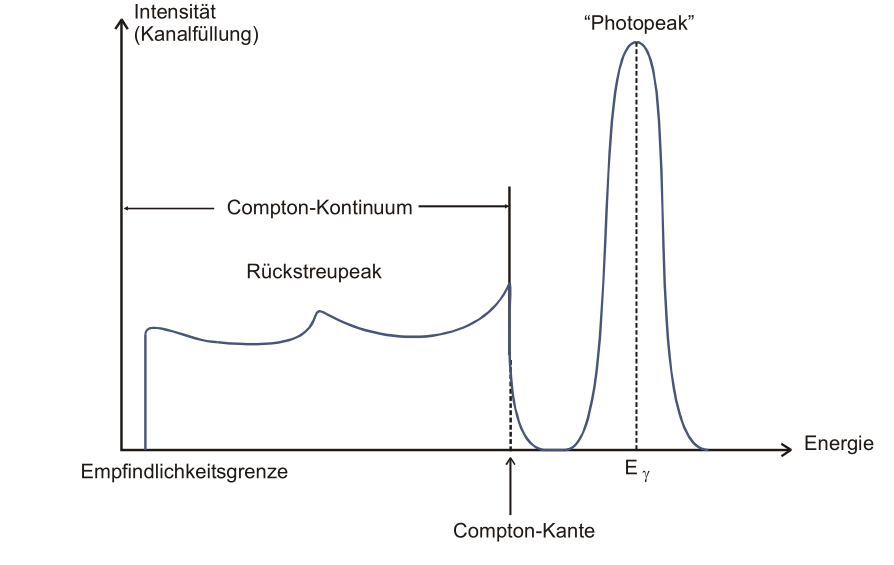
\includegraphics[width=\textwidth]{content/skizzen/idspektrum.png}
  \caption{Zu messendes Spektrum eines monochromatischen Gamma-Strahlers \cite{sample}.}
  \label{fig:idealspektrum}
\end{figure}
\FloatBarrier
Ein wichtiger Zusammenhang bei der Untersuchung der Spektrallinien eines Gamma-Strahlers ist der für
die Zählrate

\begin{equation}
  \label{eqn:effizienz}
  z = \frac{\Omega}{4\cdot \pi} \cdot A \cdot W \cdot Q .
\end{equation}
Dabei bezeichnet $\Omega$ den Raumwinkel der mit dem Detektor beobachtet werden kann, $W$ die
Emmissionswahrscheinlichkeit für eine ausgewählte Linien des betrachteten Strahlers und $Q$ die
Effizienz des verwendeten Detektors. Die Effizienz gibt an, wie wahrscheinlich es ist ein Messergebnis für eine ausgewählte
Energie zu erhalten.

\cite{sample}
